%\subsection{Directed Graphs}
Directed graphs arise in many settings. For plotting a large graph, like follower-following relationships in a social network, you might be best served making use of packages like networkx and nxviz. In other cases, you might do better working by hand. The \link{https://graphviz.readthedocs.io/en/stable/index.html}{graphviz} library is one possible solution. Here, we'll work directly with matplotlib. One directed graph use case might be in illustrating the directed acyclic graph (or DAG) representing a causal theory. In the directed acyclic graph framework (mostly associated with Judea Pearl's work in causal inference), a directed edge from $X$ to $Y$ means $X$ causes $Y$, at least in part. This lends itself well to plotting. Below we'll make a plot, using \code{plt.Circle()} to draw nodes and and creating edges with \code{ax.annotate()}.

Here, we create the nodes as circle objects and then draw the edges using \code{ax.annotate()}. Below, the circular nodes are created with the function \code{make_node()}. Then, the directed edge is drawn with \code{directed_edge()}. This doesn't allow for an edge from one node back to itself. 

\pyfile{dag-node.py}

\pyfile{dag-edge.py}

The DAG plotted below describes the theory that the persuasiveness of an argument is caused by its logical soundness and the decibel level at which it is communicated. 

\pyfile{dag-argue.py}

\begin{center}
    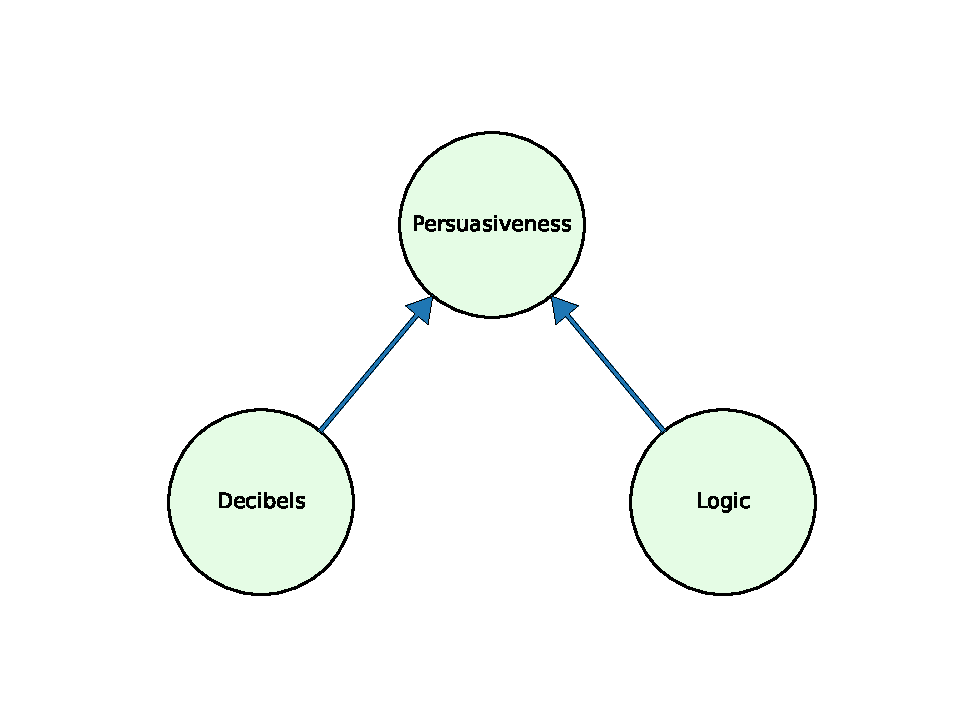
\includegraphics[width = 0.7\textwidth]{figures/poetryplots/dag-argue.pdf}
\end{center}
